\section{Introduction}
The development and research of compressed sensing applied to a single pixel camera (SPC) is a relative new area in signal processing with the first functioning camera architecture in 2006. Since then numerous improvements and methods have been proposed how to capture images. In this section a introduction to the SPC architecture and a brief introduction of compressed imaging is presented followed by the aim, research questions and thesis outline. 

\subsection{Compressive sensing \& imaging}
Compressive sensing is a new sampling strategy which reconstructs a compressible or sparse signal by finding solution to undetermined linear system. Two constraints need to be fulfilled to apply compressed sensing sampling: the sampled signal needs to be spares in some basis e.g. Fourier or gradient, the second condition is that the measurement matrix must be incoherent with the sparse transform. The characteristic  undetermined linear system in CS is defined as $ \mathbf{y} = \mathbf{\phi}\mathbf{x}$ where $\mathbf{y}$ contains the measurements from the measurement matrix $\mathbf{\phi}$ sensing the signal $\mathbf{x}$. In figure~\ref{fig:CS_eq_sys} such linear equation system is shown.

\begin{figure}[H]
	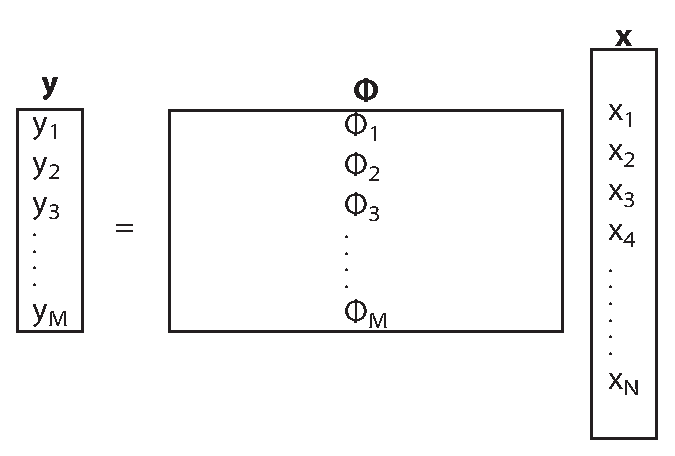
\includegraphics[scale=0.5]{gfx/CS_eq.eps}
	\caption{CS undetermined linear system}
	\label{fig:CS_eq_sys}
\end{figure}



Scientists at Rice university in Texas, USA realized that the new method could be used to create a new camera architecture with a single photo diode in the sensor, the single pixel camera was born and thus a new sub field of compressed sensing was created called compressive imaging.\\[0.1in] 

To be able to apply CS to imaging in the first place the constraints in CS needs to hold for images as well. The first requirement is that the signal needs to be compressible or sparse in some basis which natural images is known to be because they can be compressed using for example JPEG (Descrete cosine transform), JPEG2000 (Wavelet). The second constraint is that the measurement matrix must be incoherent with the sparse transform which for example white noise or some structure with the same property as white noise.\\[0.1in]

\subsection{System architecture}
The SPC in this master's thesis was designed with reflecting telescope optics to act as a lens to focus the scene. As seen in figure~\ref{fig:system_overview} light from the scene enters through the aperture in the camera where the primary mirror focus the light the via the secondary mirror onto the DMD. To this point, the SPC works like a conventional camera with the  with the difference 
the image sensor where the DMD i placed.

 where the DMD sits would be a picture sensor in a conventional camera and this is where the two cameras differ. 

 camera arcitecture was 
The system architecture is basically the same as a regular camera with two major differences. 

\begin{figure}[H]
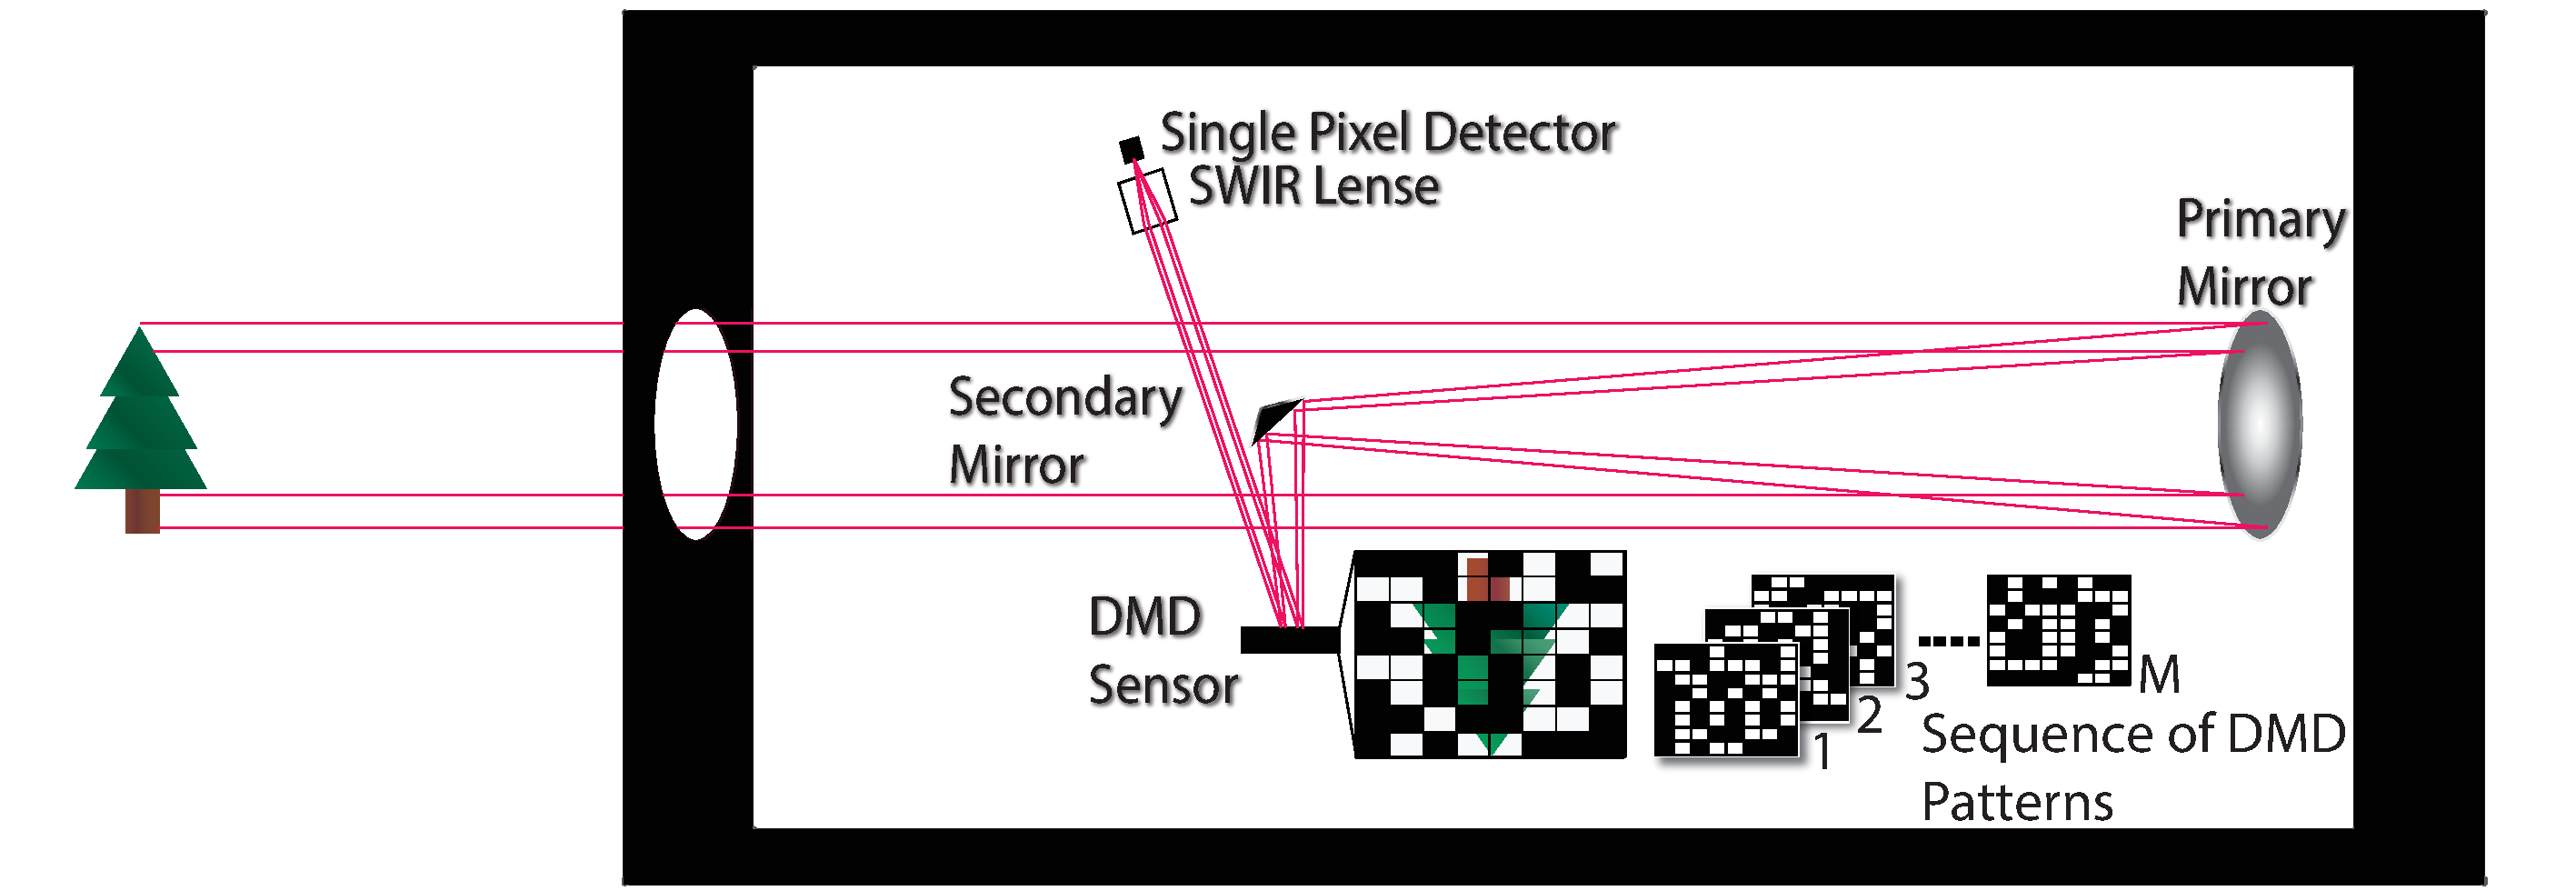
\includegraphics[width = \linewidth]{gfx/System_gif.eps}
	\caption{System overview}
	\label{fig:system_overview}
\end{figure}	

 

\begin{itemize}
\item Why?
\item Compress before the images is taken
\item Cheaper and in some cases only possible case to go to larger resolutions
\item It is more effective then scanning each pixel one by one because the one need to do N samples.
\end{itemize}





\subsection{Measurement matrix}

\subsection{Reconstruction methods}


\subsection{Aim} 
What image quality can be achieved in natural images captured with a single pixel camera in daylight using state of the art methods?  


\subsection{Research questions} 
\label{sec:RQ}
\begin{itemize}
    \item How can the quality of images reconstructed by CS or a SPC be evaluated?
    \item What is the state of the art method to capture and reconstruct images using a SPC architecture?
    \item What image quality is achieved using state of the art methods applied to the SPC?
\end{itemize}


\subsection{Limitations}
\begin{itemize}
    \item The hardware rig provided by FOI
    \item 
\end{itemize}



\subsection{Thesis outline}
